% !TEX root = main.tex
\chapter{Experimental Results}\label{cha:exp_result}
\section{Setup}\label{sec:setup}
The results in Table~\ref{tab:comp_h} and \ref{tab:comp} reveal, in terms of performance, stability and implementation considerations, two good candidates. The \abbrIRC as a stand-alone control approach and the \abbrRFDC as a harmonic cancellation add-on. Due to time limitations, only the \abbrRFDC was selected to be implemented in this thesis.

The experiments presented in this chapter has been conducted on the rotational stage described in Section~\ref{sec:rotational_stage}. A National Instruments \abbrPXI was used to communicate with the crystal collimator and the rotational stage, responsible for acquisition and control. The \abbrPXI drives the rotational stage by applying a voltage between -1 and 7.5 V that passes through a linear amplifier with a gain of \unit{20}{\volt/\volt} resulting in an input signal ranging from -20 to 150 V. The analogue output has resolution of \unit{10}{\micro\volt}. The linear position was measured by a Linear Variable Differential Transformer (\abbrLVDT) and the resolver in the stepping motor giving a linear resolution of \unit{5}{\micro\meter}. The angle of the rotational head was measured by an interferometric system (shown in Figure~\ref{fig:rotationalstage-side}) giving a theoretical angular resolution of \unit{22}{\pico\radian}. During the acquisitions, the linear stage has been in its operating position (3 mm in from its inner position) and the rotational stage has been in 6.2 mrad or 6.5 V.

\subsection{Implementation}
The control loop consisting of the original controller described in Section~\ref{sec:presentControlApproach} was executed on the \abbrPXI with an updating frequency of \unit{2}{\kilo\hertz}. The \abbrRFDC was implemented using LabVIEW and added to the existing control loop. The graphical user interface (\abbrGUI) that was created to operate the cancellation is shown in Figure~\ref{fig:gui}.

\begin{figure}[h]
  \centering %crop: left bottom right top
  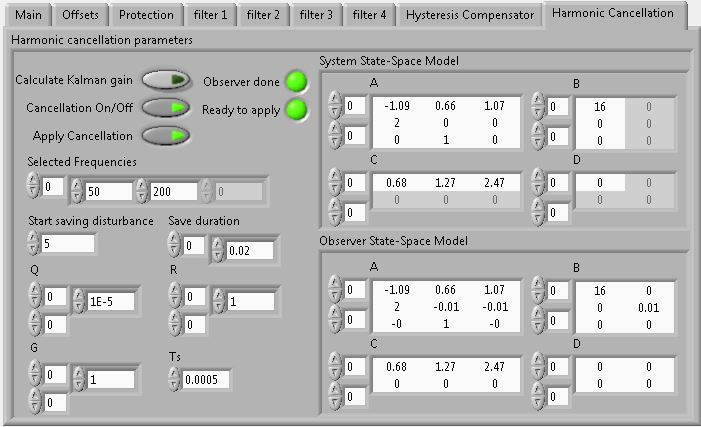
\includegraphics[width=0.8\textwidth]{fig/HC_gui}
  \caption{\label{fig:gui}Graphical user interface of the \abbrRFDC implementation.}
\end{figure}

As seen in the \abbrGUI the method requires a system model, specification of the selected frequencies, a time after initialization when the observer shall start and how long it should observe. This time must, for efficient cancellation, be a multiple of the selected disturbance period time. In the initialization phase the observer model is calculated by pressing \emph{Calculate Kalman gain}. The calculations are based on the system model and the specified tuning parameters. Cancellation is initialized by pressing the \emph{Cancellation ON/OFF}, which starts the observation. \emph{Observer done} indicates when the observation has finished and \emph{Ready to apply} when the cancellation is ready to be applied.

\section{Cancellation Verification}
The cancellation effectiveness has been evaluated in a number of different benchmarking test both in open and closed loop. Single disturbance cancellation was benchmarked by canceling an artificial disturbance added to the system by a shaker. The shaker consist of a piezoelectric actuator mounted in a prestressed structure, which generates oscillations according to the applied AC voltage. Single disturbance cancellation was also benchmarked with real environmental harmonic disturbances that was not generated by the shaker. A small test with a disturbance created and inserted directly in the code was also done to show that the algorithm did not contain any phase shifting errors. Finally the approach was tested for cancellation of multiple frequency components simultaneously.

\subsection{Single Disturbance}
The \abbrRFDC was first evaluated in open loop with single harmonics generated by the shaker. In the first test the shaker was set to generate an 80 Hz disturbance (amplitude set to 300 mV). Data was then acquired with and without the disturbance cancellation algorithm active and the result is presented in Figure~\ref{fig:fft_openloop_80} and Figure~\ref{fig:yl_openloop_80} which show the cancellation performance in time and frequency domain, respectively. Note that the acquisitions where taken successively and detrended to mitigate the creep effect. As seen in the figures, the \abbrRFDC has reduced

\begin{figure}[h!]
  \centering %crop: left bottom right top
  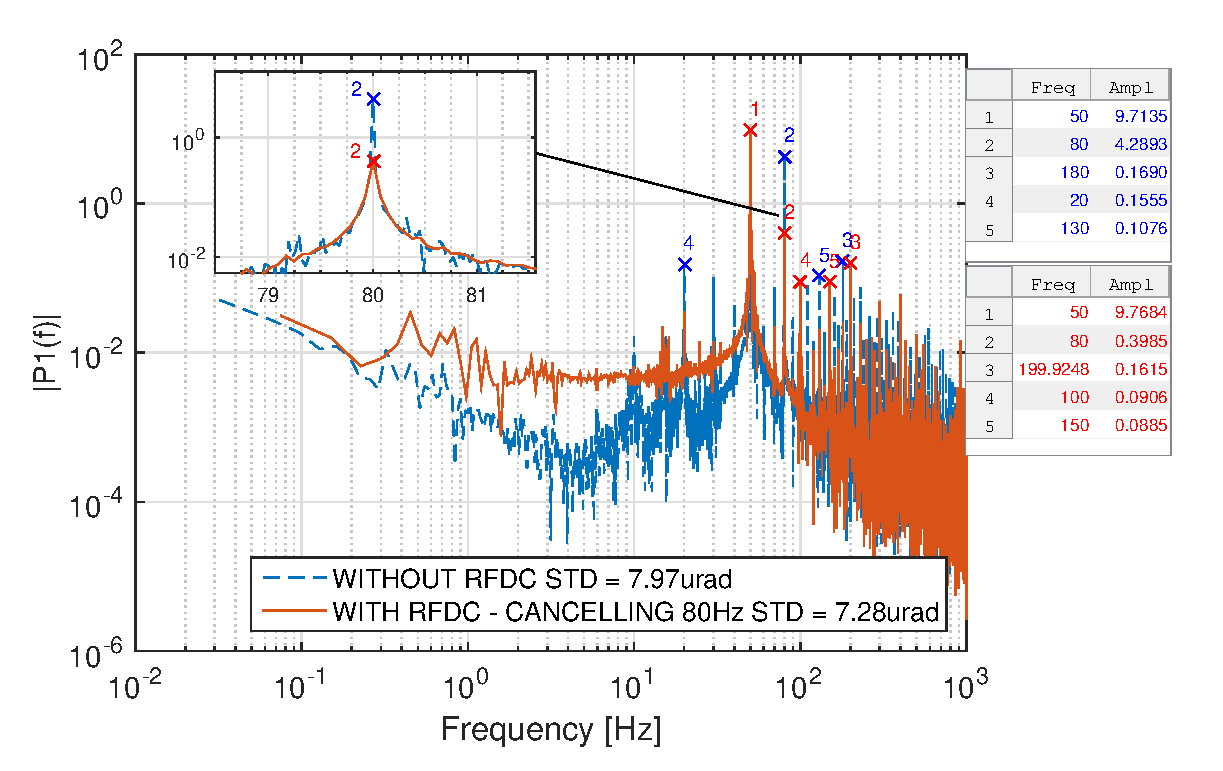
\includegraphics[width=0.85\textwidth, trim=0cm 0cm 0cm 0cm, clip=true]{fig/matlab/fft_openloop_ext_disturbance_80Hz_with_zoom}
  \caption{\label{fig:fft_openloop_80} \abbrFFT of the yaw angle response acquired in open loop with and without the \abbrRFDC active. Cancellation of the 80 Hz component generated by the shaker. The table to the right of the figures shows the amplitude of the 5 highest resonance peaks displayed in descending order.}
\end{figure}

\begin{figure}[h!]
  \centering %crop: left bottom right top
  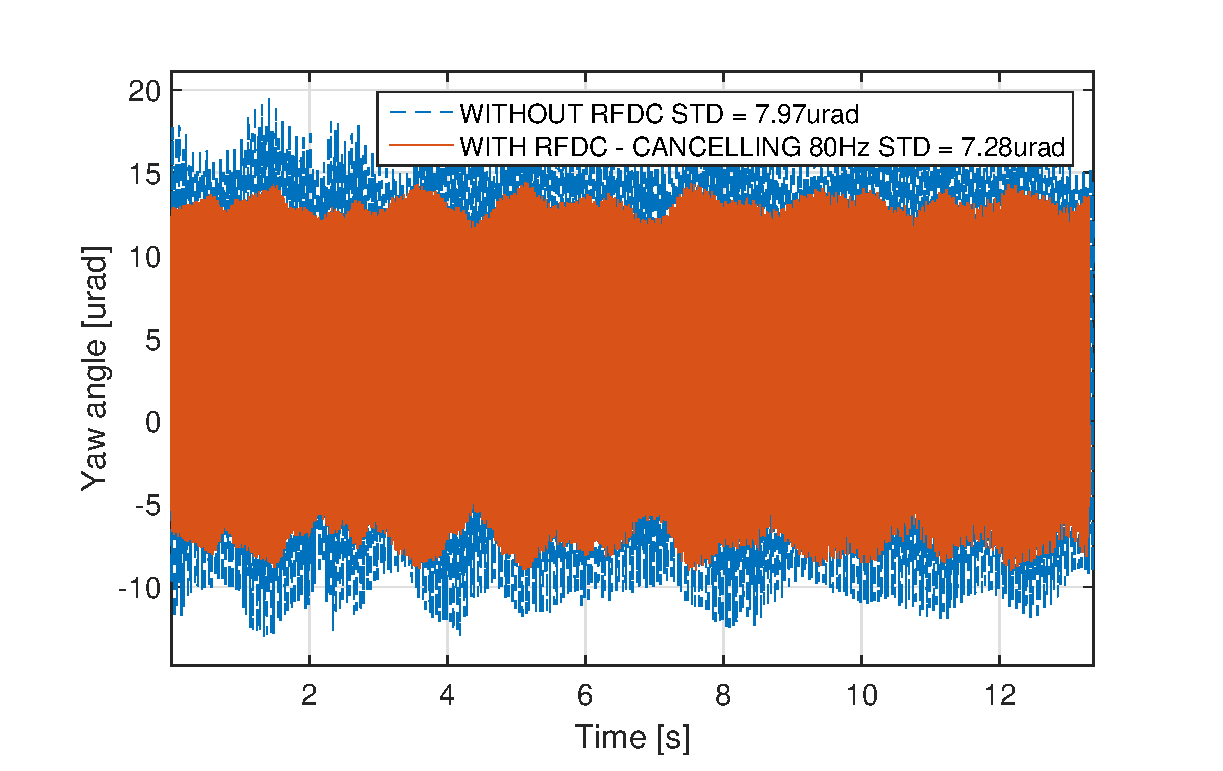
\includegraphics[width=0.8\textwidth, trim=0cm 0cm 0cm 0.7cm, clip=true]{fig/matlab/yl_openloop_ext_disturbance_80Hz}
  \caption{\label{fig:yl_openloop_80} Open loop response showing the development of the yaw angle over time, with and without the \abbrRFDC active. Cancellation of the 80 Hz component generated by the shaker.}
\end{figure}
\noindent
the 80 Hz component by 90\% of its original amplitude. The standard deviation of the signal in Figure~\ref{fig:yl_openloop_80} was reduced by more than 8\% due to the significance of the 80 Hz resonance peak.

Similar tests were performed with the controller in closed loop. The performance of the \abbrRFDC is shown in Figure~\ref{fig:fft_closedloop_80}, where the \abbrRFDC has reduced the 80 Hz component by 76\% of its original amplitude.

\begin{figure}[h!]
  \centering %crop: left bottom right top
  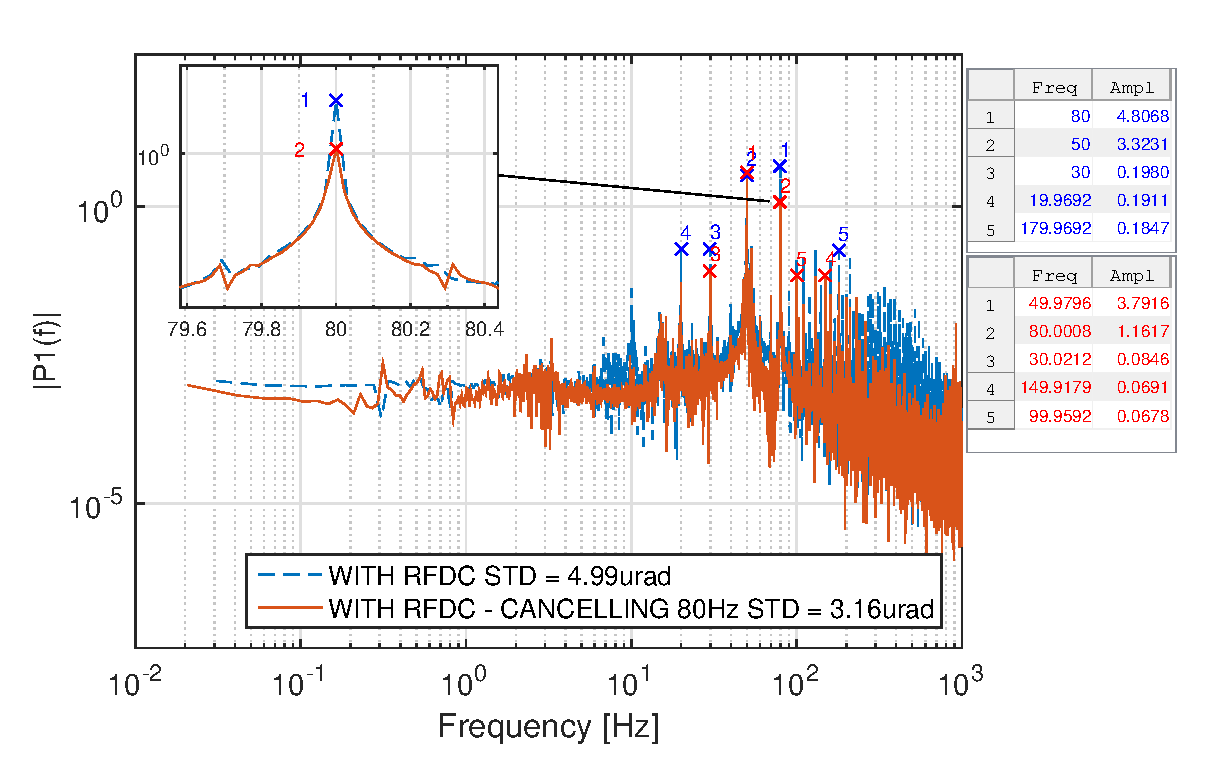
\includegraphics[width=0.85\textwidth]{fig/matlab/fft_closedloop_ext_disturbance_80Hz_with_zoom_2}
  \caption{\label{fig:fft_closedloop_80} \abbrFFT of the yaw angle response acquired in closed loop with and without the \abbrRFDC active. Cancellation of the 80 Hz component generated by the shaker.}
\end{figure}

\begin{figure}[h!]
  \centering %crop: left bottom right top
  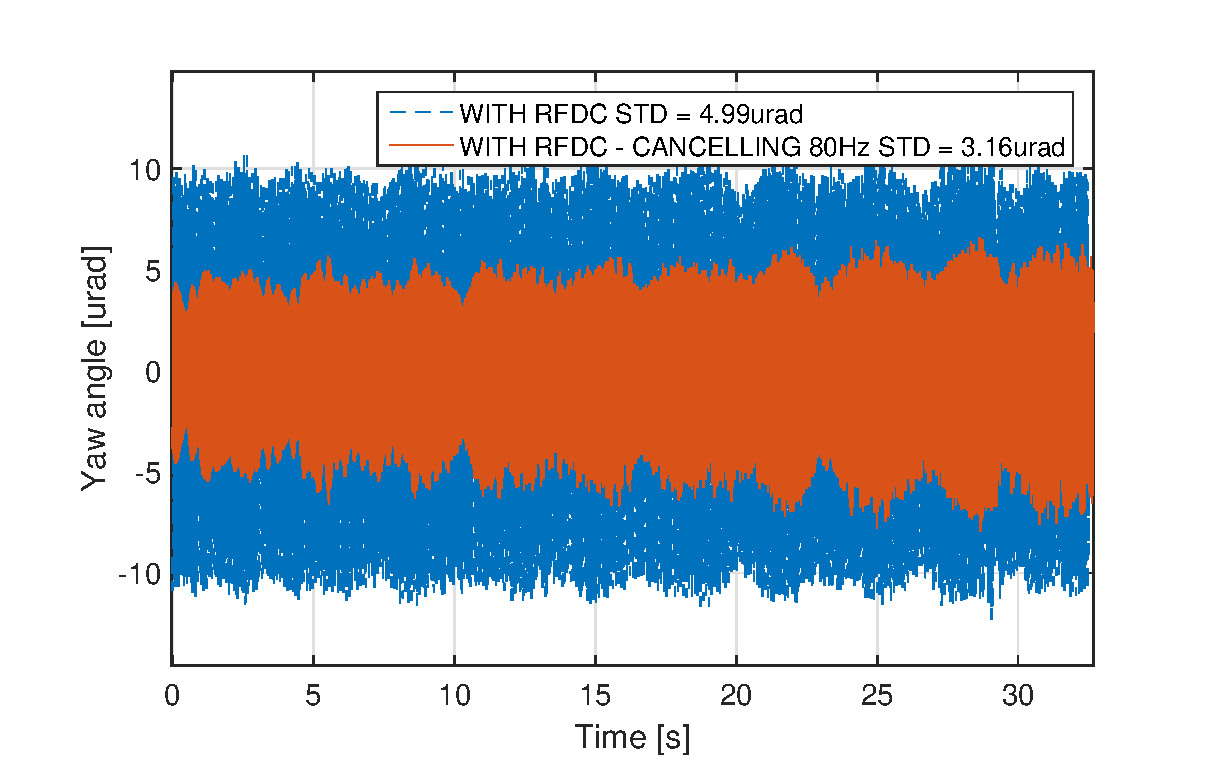
\includegraphics[width=0.8\textwidth, trim=0cm 0cm 0cm 0.7cm, clip=true]{fig/matlab/yl_closedloop_ext_disturbance_80Hz_2}
  \caption{\label{fig:yl_closedloop_80} Closed loop response showing the development of the yaw angle over time, with and without the \abbrRFDC active. Cancellation of the 80 Hz component generated by the shaker.}
\end{figure}

Figure~\ref{fig:fft_closedloop_80} also reveals a small inclination of the yaw angle evolving over time, i.e. the attenuation loses effect. In fact, looking over a larger period of time, the effect is oscillating. This effect is known as the "beat effect" and discussed further in Section~\ref{subsec:longterm}.
To further verify the performance, similar tests were also performed without the shaker applying an external disturbance. The selected disturbance was now identified by taking closed loop measurements to find dominating frequencies not attenuated by the controller itself. The 50 Hz was identified to be the most dominating component as shown in the series without the \abbrRFDC active in Figure~\ref{fig:fft_closedloop_50}. This frequency was selected and attenuated by the \abbrRFDC, resulting in a reduction of 51\% of the 50 Hz component's original amplitude. The attenuation of the 50 Hz component improved the overall yaw angle accuracy as shown in Figure~\ref{fig:transient_closedloop_50}, where the activation transient is captured.

\begin{figure}[h]
  \centering %crop: left bottom right top
  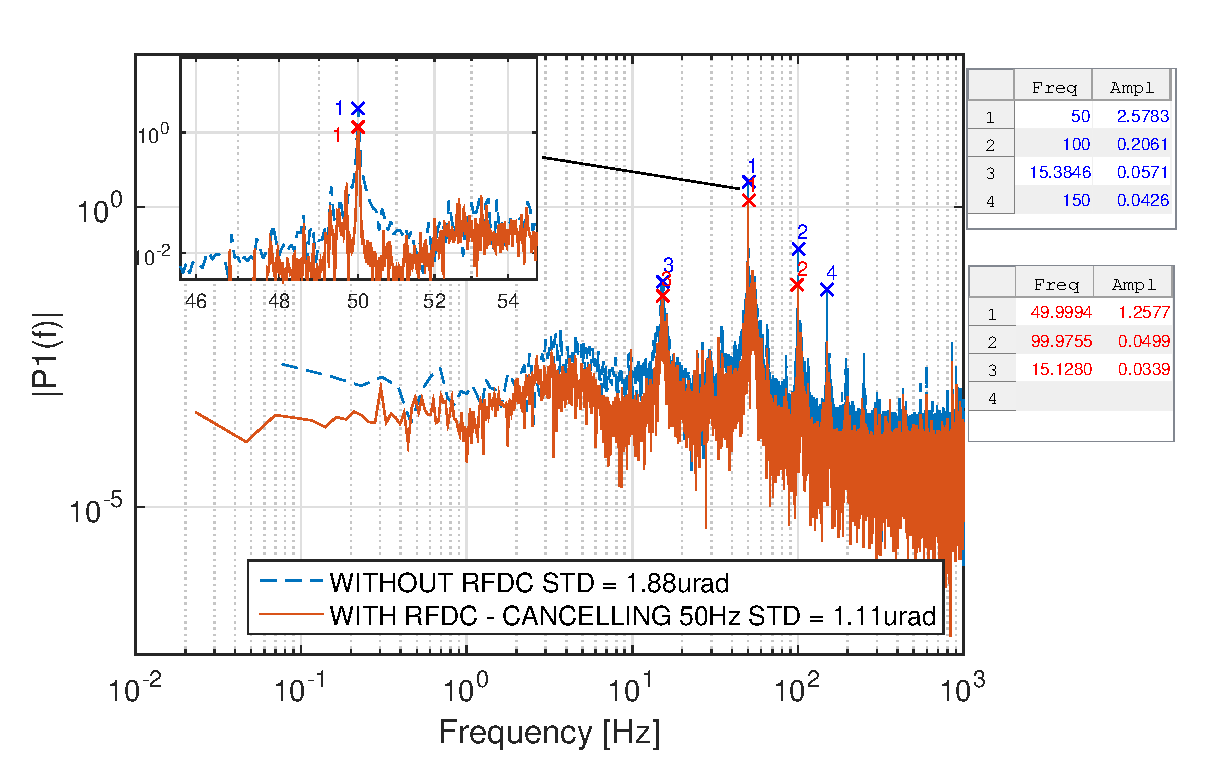
\includegraphics[width=0.85\textwidth]{fig/matlab/fft_closedloop_50Hz}
  \caption{\label{fig:fft_closedloop_50}\abbrFFT of the yaw angle response acquired in closed loop with and without the \abbrRFDC active. Cancellation of the 50 Hz component originating from environmental disturbances.}
\end{figure}

\begin{figure}[h]
  \centering %crop: left bottom right top
  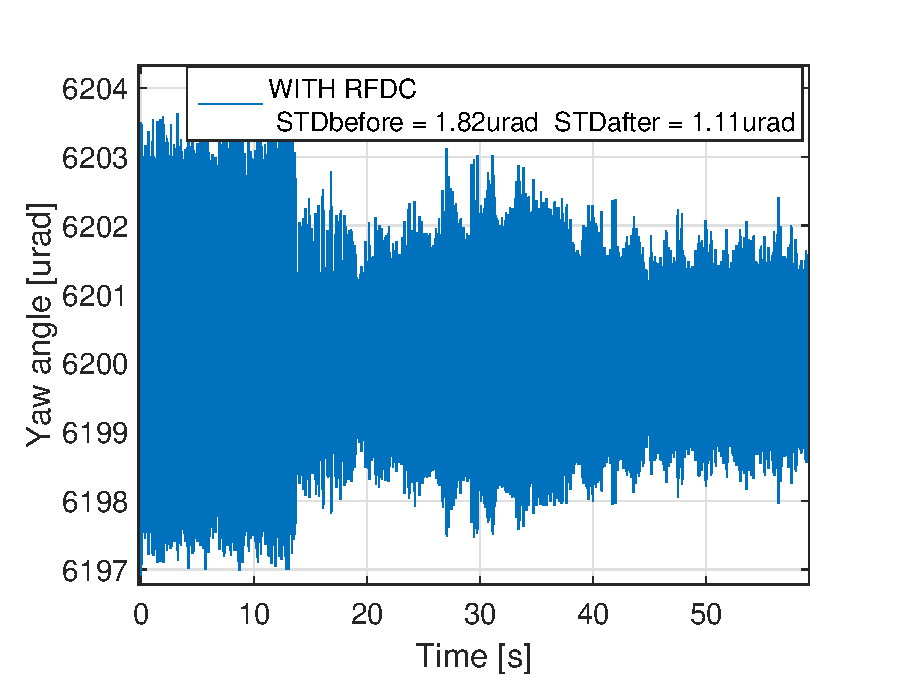
\includegraphics[width=0.8\textwidth]{fig/matlab/transient_closedloop_50Hz}
  \caption{\label{fig:transient_closedloop_50}Closed loop transient showing the response of the activation of the \abbrRFDC. Cancellation of the 50 Hz environmental disturbances.}
\end{figure}

\FloatBarrier
\subsection{Multiple Disturbances}
The cancellation of several disturbances simultaneously was verified by trying to cancel out a 50 Hz component originating from environmental disturbances in the laboratory and a 80 Hz generated by the shaker. Figure~\ref{fig:mult5080} shows the \abbrFFT of the first 10 seconds before and after the cancellation is applied. More data was acquired during the measurement but since the the system suffers from the "beat effect" only the first 10 seconds were picked out in order to show the controller ability. During this period of time the 50 Hz component was reduced by 75\% and the 80 Hz component by 66\% as seen in the figure and its corresponding tables.

The major advantage with the \abbrRFDC is that it has the ability to select specific frequencies. Since the 50 Hz component is the most dominating disturbance in the system, one could expect that when the 50 Hz is suppressed efficiently, also several other components might be attenuated. To prove that the \abbrRFDC has this capability of canceling frequencies without affecting others, another test was performed only canceling the 50 Hz component. The result can be seen in Figure~\ref{fig:mult50no80}, where it is obvious that the 80 Hz component is not affected by the cancellation of the 50 Hz component.

\begin{figure}[h]
  \centering %crop: left bottom right top
  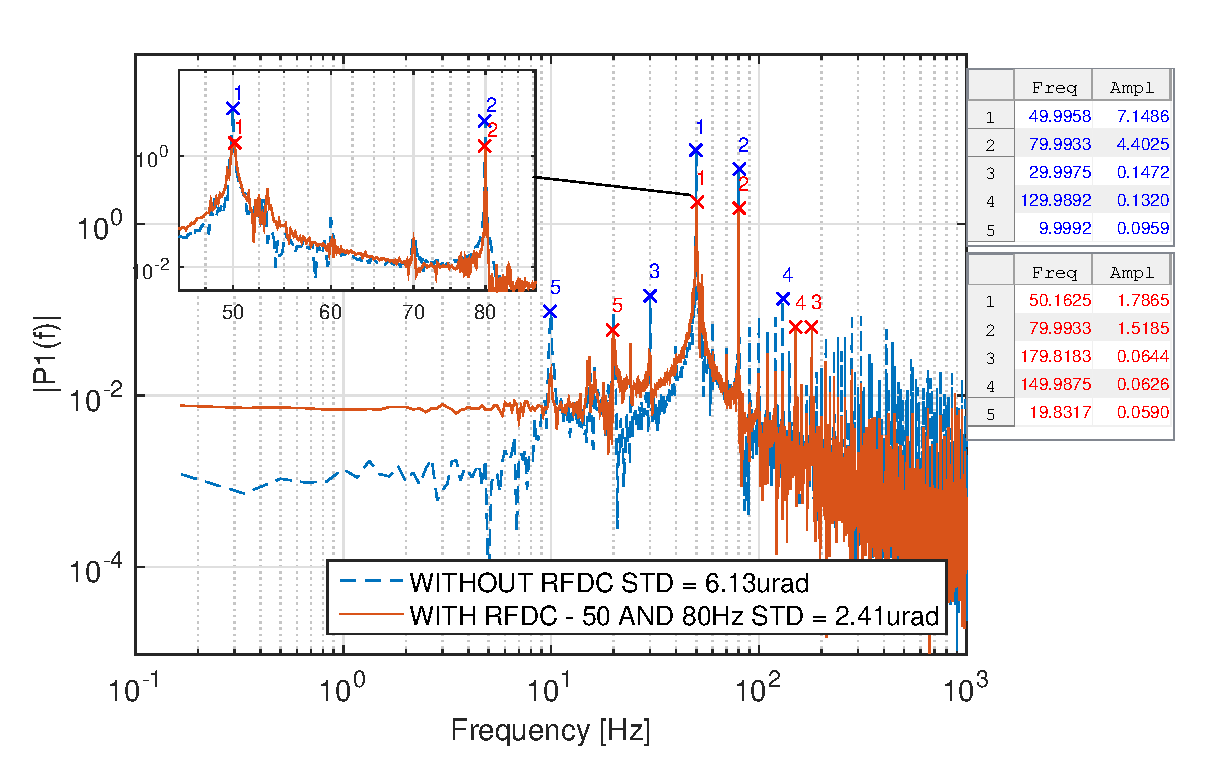
\includegraphics[width=0.85\textwidth]{fig/matlab/mult_50_80_closed_loop}
  \caption{\label{fig:mult5080} Multiple cancellation in closed loop of the 50 and the 80 Hz component. The plot is based on a 10 s long acquisition.}
\end{figure}

\begin{figure}[h]
  \centering %crop: left bottom right top
  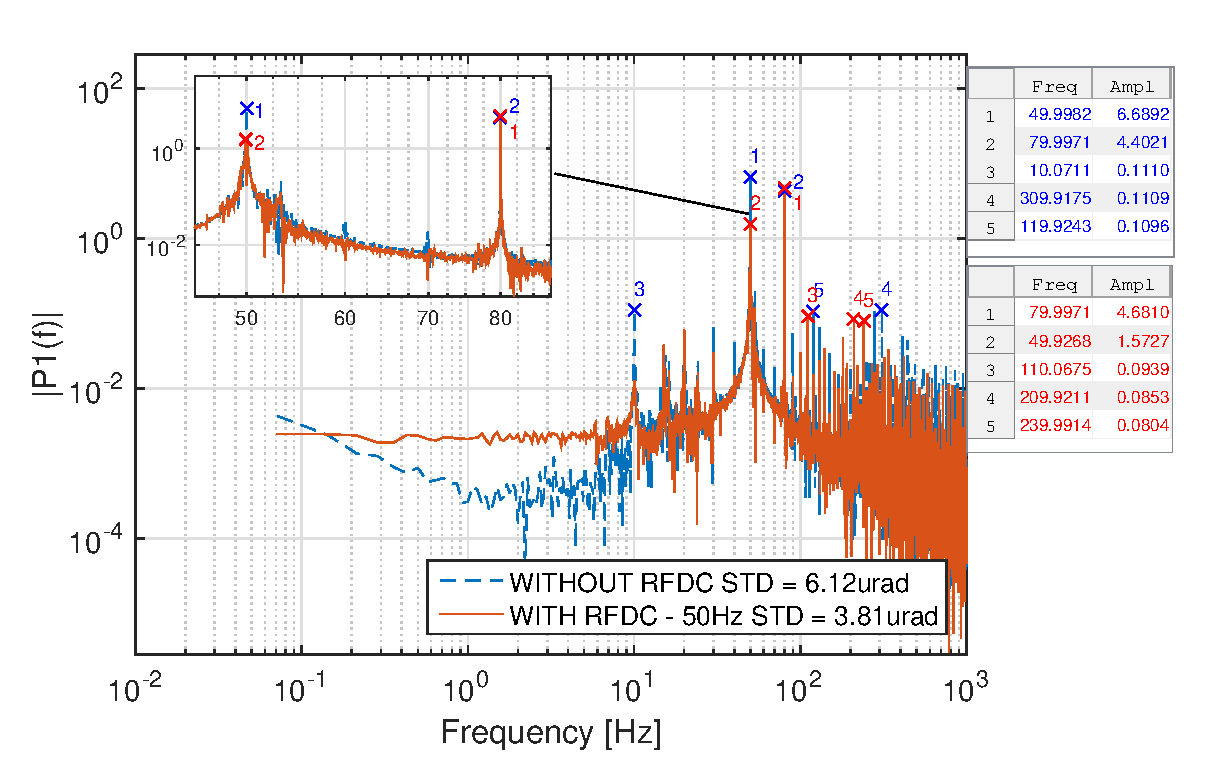
\includegraphics[width=0.85\textwidth]{fig/matlab/mult_50_selected_closed_loop}
  \caption{\label{fig:mult50no80} Cancellation in closed loop of the 50 Hz without affecting the 80 Hz component.The plot is based on a 10 s long acquisition.}
\end{figure}

\FloatBarrier
\subsection{General Findings}\label{subsec:longterm}
The capturing time, should, if possible be kept as short as possible in order to prevent modeling low frequency behavior. For low frequency disturbance cancellation, a bandpass filter could be considered to be included. Figure~\ref{fig:bandpass_imp} shows the \abbrFFT of the replicated disturbance signal. Optimally this should solely contain the selected frequency and no other components, but as seen in (a) this is not the real case. The effect of an inclusion of a bandpass filter is shown in (b), where the 15 Hz components is filtered out from the other low frequency components. The filter is designed with care to keep zero phase shift for 15 Hz components. However, this filter includes phase shift for all other components including the 50 Hz which has shown to imply in a worsened overall tracking accuracy.

\begin{figure}[h!]
  \centering %crop: left bottom right top
  \subfloat[][Without bandpass filter]{
  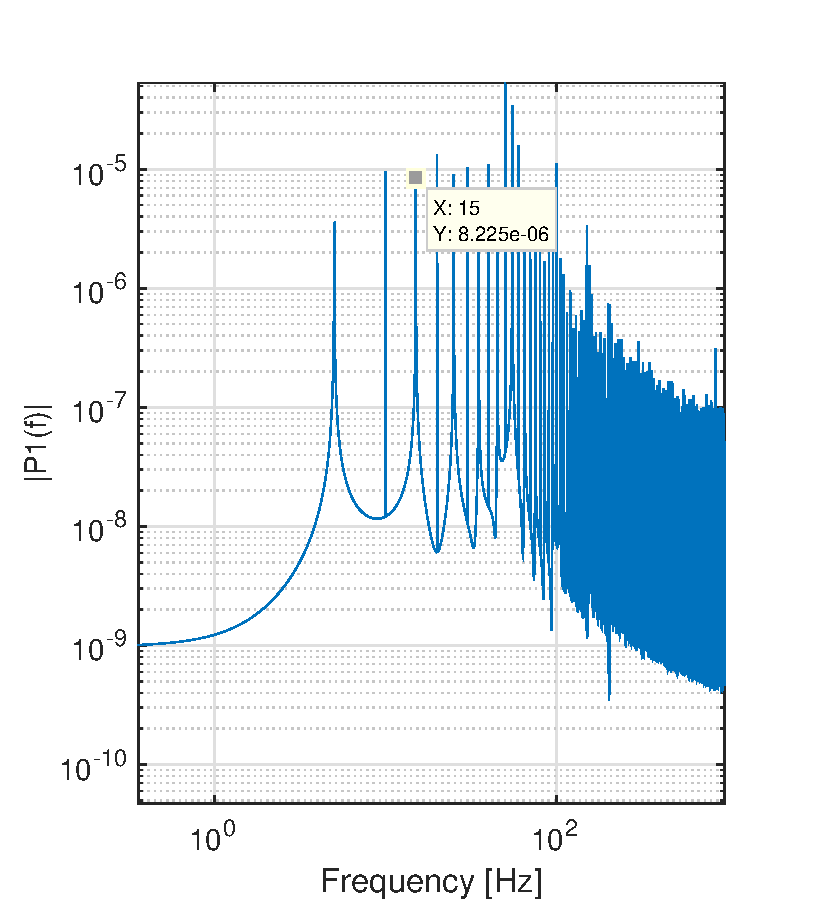
\includegraphics[width=0.46\textwidth, trim=0cm 0cm 0.8cm 1.1cm, clip=true]{fig/matlab/effect_of_bandpass}}
  \qquad
  \subfloat[][With bandpass filter]{
  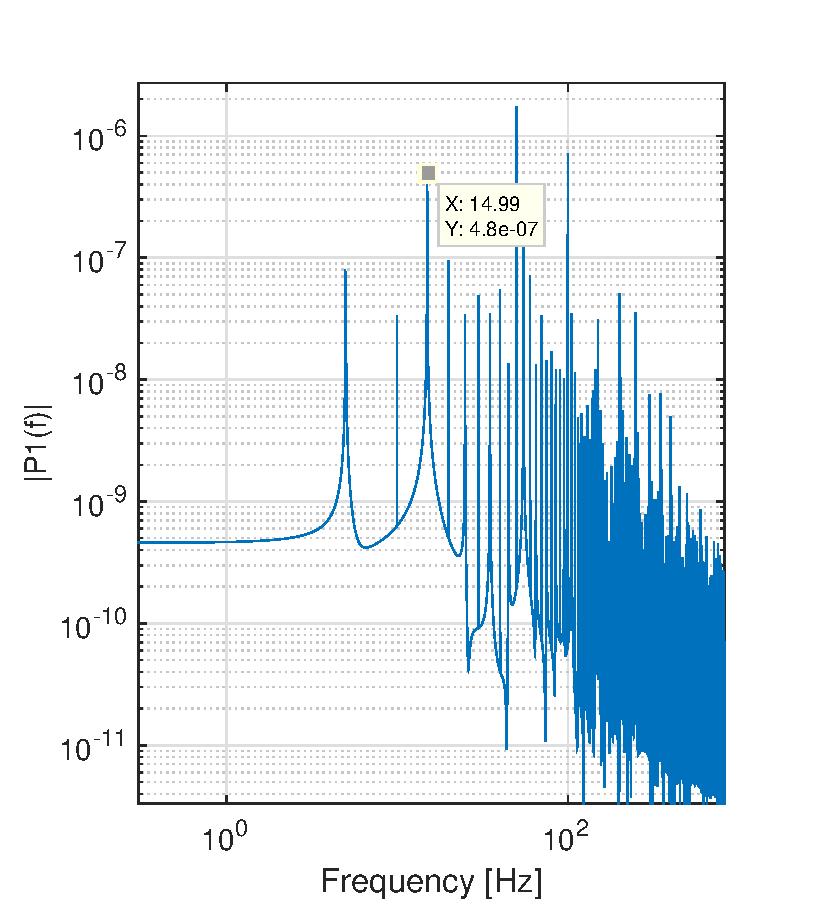
\includegraphics[width=0.46\textwidth, trim=0cm 0cm 0.8cm 1.1cm, clip=true]{fig/matlab/effect_of_bandpass2}}
  \caption{\label{fig:bandpass_imp} Effect of filtering the observed disturbance model. The figure shows the \abbrFFT of the observed disturbance model where (a) shows the original signal and (b) the filtered signal.}
\end{figure}
\FloatBarrier
An oscillating effect in the cancellation performance was observed during the measurements. This is known as the "beat effect" and explained in Section~\ref{subsec:beat}. The effect is obvious in Figure~\ref{fig:beateffect}, where the 50 Hz component is only canceled a fraction of the total acquisition time. According to \eqref{eq:beat}, the envelope frequency is half the difference between the two frequencies. The envelope in Figure~\ref{fig:beateffect} has a period of 50 s giving a beat frequency of 0.04 Hz. To verify that the beat effect was not induced by the algorithm itself, a simple test with two artificial disturbances were performed. Two disturbances were created and injected directly in the program. These frequencies were then set to be canceled by the \abbrRFDC. The result is shown in Figure~\ref{fig:nobeat} where the standard deviation of the yaw angle displacement can be seen with and without cancellation. The cancellation is here kept constant over 2 minutes, showing no sign of the beat effect.

\begin{figure}[h!]
  \centering %crop: left bottom right top
  \subfloat[][Yaw angle displacement]{
  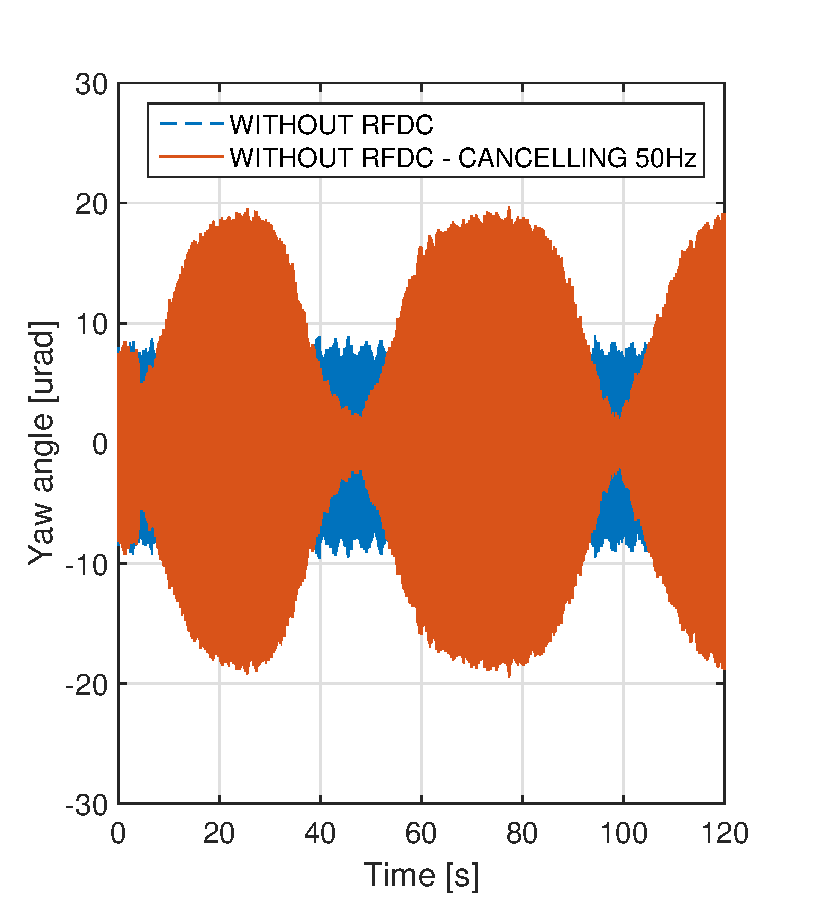
\includegraphics[width=0.46\textwidth, trim=0cm 0cm 0.8cm 0.8cm, clip=true]{fig/matlab/beat_effect_yl}}
  \qquad
  \subfloat[][Standard deviation of yaw angle displacement]{
  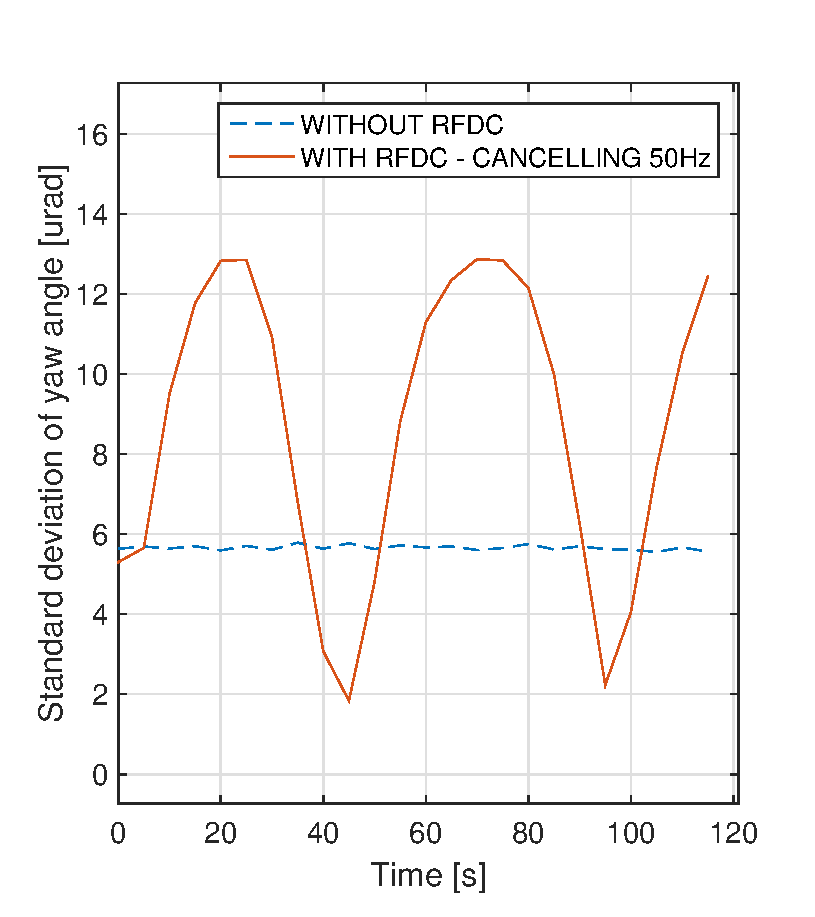
\includegraphics[width=0.46\textwidth, trim=0cm 0cm 0.8cm 0.8cm, clip=true]{fig/matlab/beat_effect}}
  \caption{\label{fig:beateffect} Cancellation performance in closed loop of the 50 Hz component suffering from the beat effect. The standard deviation, calculated as an average of the standard deviation of (a) every 5 s, is shown in (b).}
\end{figure}

\begin{figure}[h!]
  \centering %crop: left bottom right top
  \subfloat[][Yaw angle displacement]{
  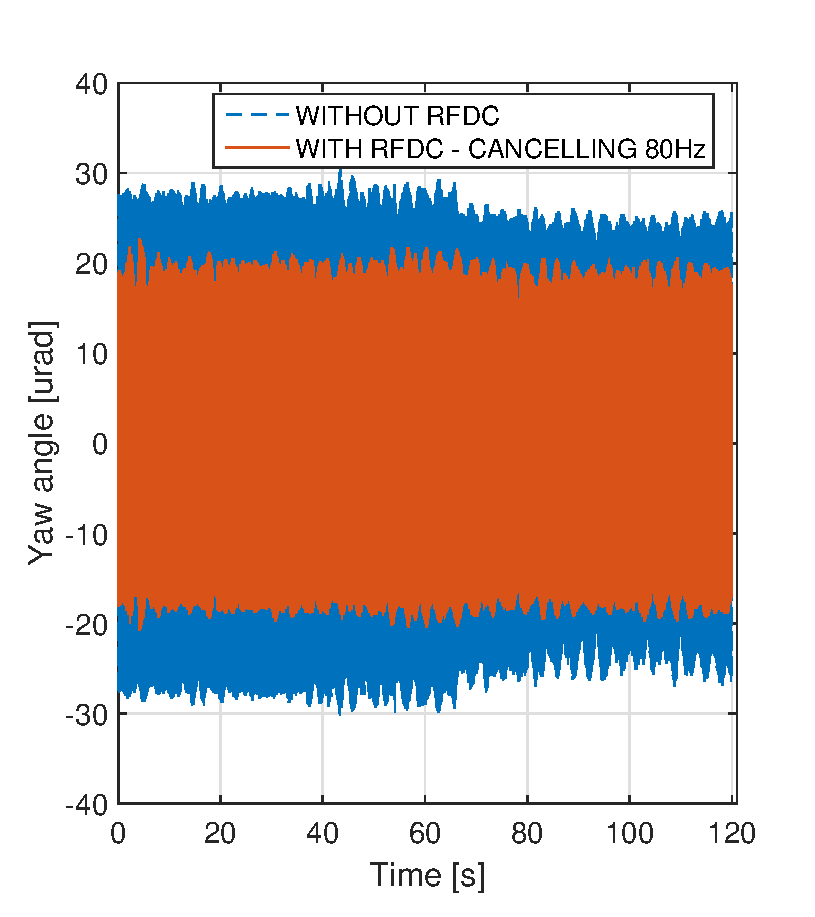
\includegraphics[width=0.46\textwidth, trim=0cm 0cm 0.8cm 0.8cm, clip=true]{fig/matlab/no_beat_effect_yl}}
  \qquad
  \subfloat[][Standard deviation of yaw angle displacement]{
  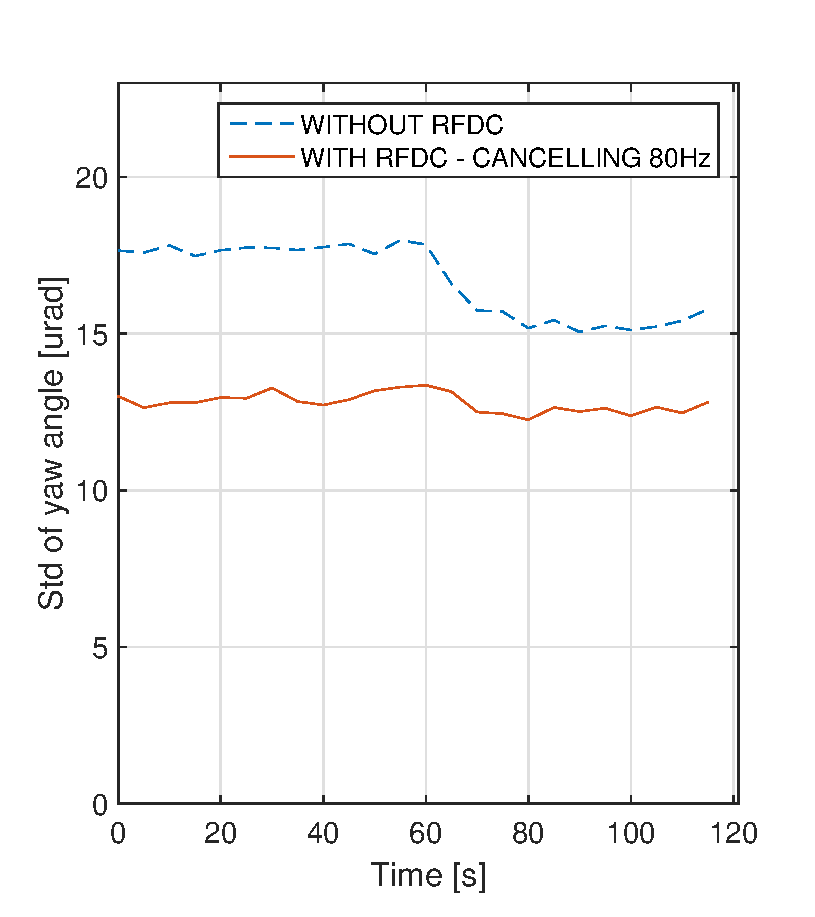
\includegraphics[width=0.46\textwidth, trim=0cm 0cm 0.8cm 0.8cm, clip=true]{fig/matlab/no_beat_effect}}
  \caption{\label{fig:nobeat}Cancellation of artificial disturbances in open loop not suffering from beat effect. The yaw angle is shown in (a) with the standard deviation in (b). The change in the data without \abbrRFDC is due to environmental changes.}
\end{figure}
\FloatBarrier
The conspicuous change in the data acquired without the \abbrRFDC active, seen at $t=$ 60 s, is due to the environmental changes that were present during the acquisition. However, this change has no impact on the results since the purpose of this test was only to verify that the algorithm provided stable cancellation.
